%%%%%%%%%
% TO DO %
%%%%%%%%%
% Expand intro
% Redo graphs from graphing program, expand scope, involve 
% More detail
% Actually describe motivation again
% Rewrite into based off previous chapters


%Don't write too much
%Write what is needed in the text
%The more you write, the higher probability of making mistakes - keep to the point
%Describe results
%Explanation after desc
%Have to be phrases that make sense/say something
%Have a purpose

\chapter{Analysis of Approach Force Curves in Colloidal Systems}
\label{chap:approach_force_curves}

This chapter aims to serve a simple goal. To provide a clear route to extract the force at contact from raw data.  As the raw unprocessed data is severely voluminous the scope of this chapter is kept to one goal, provide the data and justification for the contact forces calculated for each concentration, site and parameter. The results of this analysis is then concluded in Chapter 7, which, is free of the need to justify every data point and thus focuses on the conclusions from this data. 

This data, along with the further analysis provided in chapter 7 is expanded upon, and insights are drawn from this in turn. In order to aid readability/referenceability, this chapter focuses on the data collected during the 

\section{MFP-1D contact force derivation}

For the data collected from the MFP-1D the analytical approach to this elucidation is given in Chapter 4. This section will overview the results for the following LiCl concentrations: 0.6mM, 1.6mM, 5mM, 10mM, 25mM, 50mM, 230mM, 550mM. For each concentration multiple sites are analysed, highlighting features of each curve in preparation for analysis. 

\subsection{A note on rejected curves}

 During the process, several curves were rejected from the data set as part of the processing method, due to the large volume of curves involved in this analysis. This was either due to machine failure to engage in the surface, or due to significant noise due to mechanical failure (over-correction in piezo movement by the AFM or vibrations in the building.) While the initial curves taken on the machine were too noisy, further repeats and refinements to the procedure eventually resulted in usable curves. In some of the data collected, the impact from residual vibrations was mitigated in later datasets by operating the AFM in the night. Other improvements were found by optimising the AFM parameters  - such as tip speed, data collection rate and target force. The optimal parameters found were 0.5Hz for tip speed, setting the data collection rate to maximum and a target force of 8-12 nN. 

\begin{figure}
    \centering
    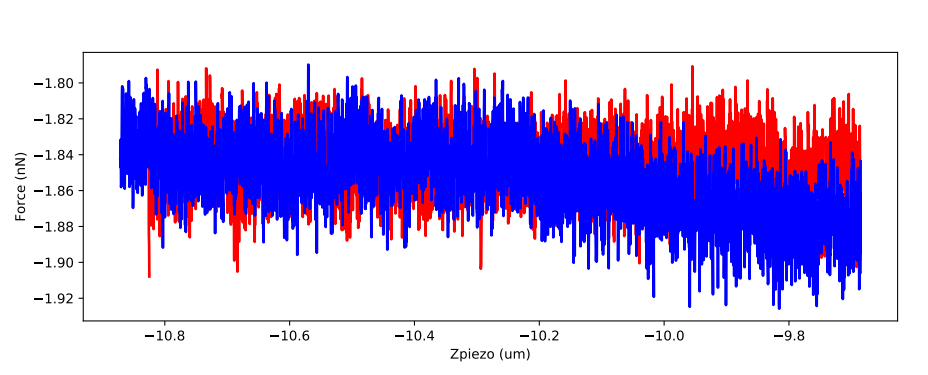
\includegraphics[width=0.65\linewidth]{chapter5/miss_error.png}
    \caption{A graph demonstrating a rejected curve. In this case the AFM failed to reach the surface for the recorded data, leading to a single up and down motion. In this case red is the approach curve and blue is the retrace curve.}
    \label{fig:miss-error}
\end{figure}

The other reason for rejected curves was due to the shift of the snapshot window providing too little data in either the approach phase or the contact phase (covered in Chapter 4). 

\subsection{Contact force calculations}

In this results section, the contact force graphs displayed represent only a subset of the total analyzed graphs, selected to illustrate the most significant aspects of the analysis procedure. The ones chosen here represent the typical majority of the curves, with outliers not reflected in the dataset. Outliers may be demonstrated, and will be commented on if presented. The remainder of the curves, not shown here, played an instrumental role in guiding the parameter optimization process for the data processing script. This process involved the review and refinement of several hundred thousand curves in order to deal with the noise intrinsic to the system. Ensuring a good fit for these curves is paramount; otherwise, one risks obtaining erratic and misleading graphs that could compromise the integrity of the data interpretation. The selection process for the resulting curves involved the exclusion of certain outliers and repeat measurements, a necessary step taken to refine the data and enhance the clarity of the observed trends. Three types of graphs were chosen for their analysis of the fitting parameters and results: the histogram of contact forces provides a statistical view of the interaction forces at the point of contact, demonstrating the range of forces across the graph. The log-linear plot of the force as a function of the Z-piezo position (in nanometers), highlighting of the separation distance between the AFM tip and the sample surface during the interaction phase. At the top of the graph the transition to the contact phase can be seen. This point of transition is the contact force. The logarithmic scale for force highlights the sensitivity of the AFM in detecting forces at the nanoscale. Finally the overall approach force curve derived from binned data presents a view of the resulting averaged force curve behavior during the approach phase. Each graph was selected for its ability to support the chosen parameters and thus the resulting contact force.

\subsection{Diversity and Range of Data Points}
Each site and corresponding graph included in Chapter 5 were selected to represent the wide range of experimental conditions explored in this study. The diversity of salt concentrations (ranging from 0.6mM to 550mM) provides a comprehensive view of how the interactions between colloidal particles change under different ionic strengths. By including data from various sites, the results shown are not biased by localized effects, but are reflective of the overall behavior of the system. This approach highlights trends across the dataset, such as the transition from repulsive to attractive forces as the salt concentration increases, which is required for understanding the underlying mechanisms governing colloidal stability.

The "shelf" feature observed in some of the following force profiles is of particular interest because it indicates a potential secondary interaction mechanism that might not be explained by traditional DLVO theory alone. The inclusion of these specific sites and graphs where the shelf feature is prominent was intentional. Highlighting this phenomenon is important because it may suggest the presence of complex surface interactions, possibly related to surface roughness or heterogeneities, which could have significant implications for the interpretation of force measurements in colloidal systems.

The presence of the shelf at different concentrations and its persistence across various sites suggest that it is not a random artifact but a consistent phenomenon that warrants deeper analysis. Including these graphs provides a more complete picture of the force interactions at play and challenges us to consider additional factors that may influence colloidal stability beyond those traditionally considered in DLVO theory. A dedicated analysis of this observation is provided later in section 8.3. This shelf feature isn't without literature precedent however, as it has been observed previously. \cite{Kilpatrick2013DirectlyProbing} \cite{guleryuz2012afm}

%0.6mM
\insertapproachfigures{5}{0.6}{1}{Site one demonstrates one of the difficulties with collecting the data at the lower ranges of the molar concentrations. As the repulsive force is over a wider range there is a smaller window captured of the contact phase. This means that when trying to fit to the curve, there is less data available to provide a solid fit.  As such, a slight bowing effect is seen in the binned average curve.
Additionally, the signal to noise ratio in this curve is significantly high compared to others, with the later graphs of higher concentrations generally having a better signal to noise ratio.

38 curves in total were processed. Of these processed curves the average contact force was 5.2 nN $\pm$ 1.5 nN.}
\insertapproachfigures{5}{0.6}{2}{Site two demonstrates the lowest observed force for this concentration, highlighting a high degree of variability between sites. However, this may be due to difficulty in finding a good fit. As the maximum contact force was capped, some of the curves ended within the contact region, or just after, limiting the number of viable curves.

13 curves in total were processed.  Of these processed curves the average contact force was 3.6 nN $\pm$ 0.3 nN.}
\insertapproachfigures{5}{0.6}{3}{Site three demonstrates an ideally fitted curve, however in the log-linear plot an irregularity is seen - the point in which the contact force area is raised up the graph. This is due to the large amount of noise seen during this interface phase, giving a large variation in the contact force histogram.

29 curves in total were processed. Of these processed curves the average contact force was 4.7 nN $\pm$ 1.4 nN.}
% ... and so on for other sites and concentrations.

%1.6
\insertapproachfigures{5}{1.6}{1}{Site one represents an good example of a typical well-behaved curve, where the processing is able to extract out a clear signal from the noise, and thus a clearly distributed contact force.

140 curves in total were processed. Of these processed curves the average contact force was 2.6 nN $\pm$ 0.6 nN}
\insertapproachfigures{5}{1.6}{2}{Site 2 demonstrates an interesting feature - a region where there seems to be two contact phases. As DLVO doesn't explain any dual barrier features this is rather unexpected. One explanation may be that as the two surfaces approach one another some aspect (for example a small topographical protrusion or a small aggregate of ions) prevents full contact between the sphere and surface, which then slips or is overcome, allowing full contact later. It is important to note that this feature is present throughout the dataset, and survived the binning and averaging process, and thus is a consistent feature in this site.

113 curves in total were processed. Of these processed curves the average contact force was 4.5 nN $\pm$ 0.5 nN}

%5
\insertapproachfigures{5}{5}{1}{Site one demonstrates a similar, but weaker feature seen in 1.6 mM site 2 observable in the log-lin plot. The overall binned fit demonstrates a suitable fit, so it remains to be a feature of this site. Equally, this site demonstrates the weakest repulsive force in the set.

128 curves in total were processed. Of these processed curves the average contact force was 2.2 nN $\pm$ 0.5 nN}
\insertapproachfigures{5}{5}{2}{Site two demonstrates the same feature, but slightly less prominent again.

110 curves in total were processed. Of these processed curves the average contact force was 3.1 nN $\pm$ 0.7 nN}
\insertapproachfigures{5}{5}{3}{Site three once again has the feature seen across all of the force curves at this concentration

114 curves in total were processed. Of these processed curves the average contact force was 3.8 nN $\pm$ 0.5 nN}

1.6 mM site 2 and 5 mM presents an interesting and repeatable shelf seen in the force profiles across all different sites. There are a number of theories as to what this feature may be. For one If the AFM tip encounters a region of the sample with a topological feature that does not mesh well with the surface it could provide the observed barrier. This feature can then hold the tip back from fully sliding down until a threshhold force determined by the surface roughness is presented. Once this threshold force is overcome it then "slips" down further into contact.

%10 2 sites
\insertapproachfigures{5}{10}{1}{Site 1 demonstrates a noisy top of the graph, which can sometimes happen when the AFM oversteers and provides too much force onto the sample.

130 curves in total were processed. Of these processed curves the average contact force was 1.8 nN $\pm$ 1.1 nN}
\insertapproachfigures{5}{10}{2}{119 curves in total were processed. Of these processed curves the average contact force was 3.8 nN $\pm$ 0.4 nN}
\insertapproachfigures{5}{10}{3}{124 curves in total were processed. Of these processed curves the average contact force was 4.4 nN $\pm$ 0.5 nN}

%25 3 sites
\insertapproachfigures{5}{25}{1}{Site 1 demonstrates a high degree of noise in the binned average curve and demonstrates towards what curves could be without the involved processing

144 curves in total were processed. Of these processed curves the average contact force was 2.2 nN $\pm$ 1.7 nN}
\insertapproachfigures{5}{25}{2}{Site 2 also demonstrates a shelf feature.

124 curves in total were processed. Of these processed curves the average contact force was 2.7 nN $\pm$ 1.1 nN}
\insertapproachfigures{5}{25}{3}{76 curves in total were processed. Of these processed curves the average contact force was 3.9 nN $\pm$ 1.5 nN}

%50 2 sites
\insertapproachfigures{5}{50}{1}{50mM both demonstrates the presence of the shelf feature, as well the contact force following the trend of decreasing over time.

104 curves in total were processed. Of these processed curves the average contact force was 3.3 nN $\pm$ 0.6 nN}
\insertapproachfigures{5}{50}{2}{105 curves in total were processed. Of these processed curves the average contact force was 2.8 nN $\pm$ 0.7 nN}

%230 2 sites
\insertapproachfigures{5}{230}{1}{230mM demonstrates the point in which the repulsive force observed is close to 0. The shelf feature observed in the 230mM data is particularly significant because it suggests a region of weak attraction following the initial contact. This feature is not consistently observed in all graphs, which could be due to variations in local surface roughness, heterogeneity in the colloidal particles, or slight differences in the approach speed of the AFM tip.

109 curves in total were processed. Of these processed curves the average contact force was 2.2 nN $\pm$ 0.3 nN}
\insertapproachfigures{5}{230}{2}{84 curves in total were processed. Of these processed curves the average contact force was 0.8 nN $\pm$ 0.4 nN}

%550 3 sites
\insertsnowflakefigures{5}{550}{1}{500mM marks the situation where the charge screen starts to overcome the electrostatic repulsion, giving way to an attractive force instead. Interestingly the shelf effect is still observed despite the attractive nature of the two surfaces.

84 curves in total were processed. Of these processed curves the average contact force was -0.3 nN $\pm$ 0.1 nN}
\insertsnowflakefigures{5}{550}{2}{107 curves in total were processed. Of these processed curves the average contact force was -0.1 nN $\pm$ 0.1 nN}
\insertsnowflakefigures{5}{550}{3}{89 curves in total were processed. Of these processed curves the average contact force was -0.1 nN $\pm$ 0.1 nN}

\section{Overall force vs LiCl concentration graph}

The forces calculated at the point of contact were subsequently plotted on a graph. For the values, the average was taken, the standard deviation was calculated by:

\begin{equation}
Stdev_{avg} = \sqrt{\frac{{x_1}^2 + {x_2}^2 + {x_3}^2}{n_{num}}}  
\label{eq:Stdevavg}
\end{equation}

Where $x$ is the site's standard deviation and $n_{num}$ is the number of sites in the calculation (i.e. where there were 3 sites, this value was 3).

 In the case of a LiCl concentration of 550 mM, the attractive force was utilized in the plot due to the alteration in the nature of the force curve.

\begin{figure}
    \centering
    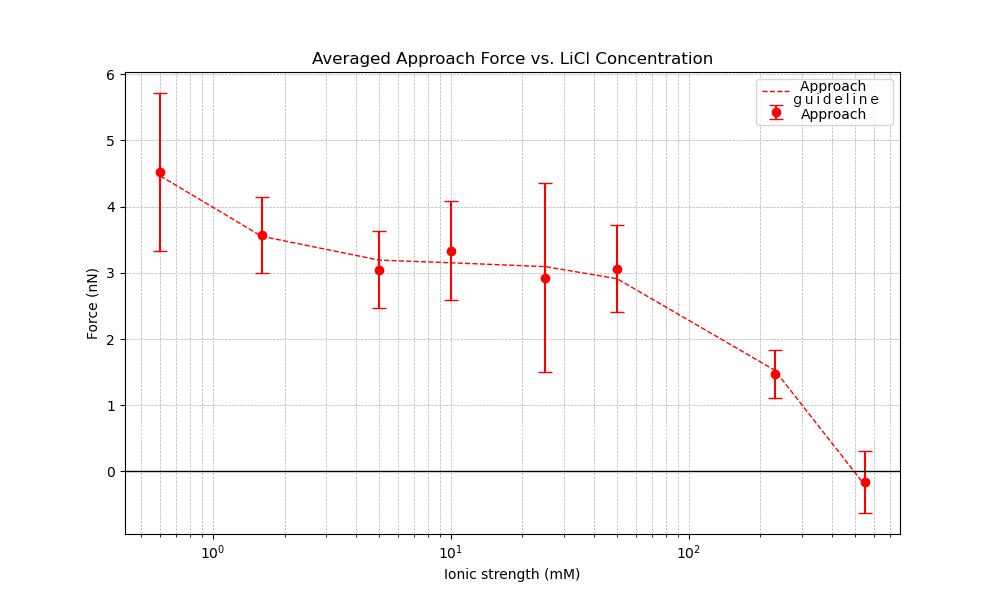
\includegraphics[width=1\linewidth]{chapter5/Average Approach.png}
    \caption{All sites' calculated force at contact with standard deviation error bars. There is an observed trend of increasing LiCl concentration leading to a decrease in repulsive force, until the repulsive force becomes attractive.}
    \label{fig:site1cont}
\end{figure}

The overall graph demonstrate the force at contact appears to decrease with increasing LiCl concentration. The reality for each of the sites is that they were exposed to different tips and different sites. As the AFM used was unable to save site locations, site 1, 2 and 3 aren't the same spacial location on the glass between salt concentrations.

An interesting observation however is in the error bars and thus the variability or uncertainty of the measurements. Larger error bars at middling concentrations, especially noticeable at 25mM, might suggest greater variability in the interaction forces measured at these points.

The dotted line was added to guide the rough direction of the plots, which indicates that as salt concentration increases, the force requires for silica particles to come into contact decreases, eventually giving way to an attraction between the particles. This is likely due to the higher salt concentrations screening the electrostatic interactions. However, another interesting aspect is an observed plataeu between 5 - 50mM ionic strengths, potentially indicating a critical ion concentration needed to disrupt the electrostatic repulsion enough in this region.

These calculated forces are then expanded upon in chapter 7, with further analysis into potential reasons as to why these trends are observed.

\section{Discussion of Force Measurements and Salt Concentration Effects}

The interaction forces between silica surfaces in electrolyte solutions have been a significant area of study in surface science, particularly in understanding the influence of varying salt concentrations on adhesion forces. The results obtained in this thesis, particularly regarding the influence of LiCl concentration on the contact forces between silica particles, align with and extend findings from previous studies such as those by Guleryuz et al. (2012) and Kostakis et al. (2006). \cite{Kostakis2006} \cite{Guleryuz2012}

Guleryuz et al. (2012) performed AFM measurements of forces between silica surfaces in the presence of NaCl and reported that increasing the salt concentration significantly reduces the electrostatic repulsion between the surfaces. This reduction in repulsion allowed for a more pronounced adhesion force as the surfaces approached closer under the influence of the van der Waals attraction. Specifically, their study showed that at higher pH levels, where the silica surface is more negatively charged, the presence of high NaCl concentrations reduced the Debye length, thereby diminishing the range of the electrostatic double-layer repulsion and resulting in a higher adhesion force. In the context of the findings presented in this Chapter, a similar trend was observed, with LiCl instead, where increasing concentrations led to a decrease in the repulsive forces and a corresponding increase in the adhesion forces measured between the silica particles. \cite{Guleryuz2012}

The work by Kostakis et al. (2006) further complements these findings by exploring the stabilization of bubbles by silica particles in high salt concentrations. They noted that at high NaCl concentrations, the surface structures, such as polysilic acid chains, collapsed, leading to a significant reduction in steric repulsion and an increase in adhesion. This observation parallels the results of Chapter 5, as it suggests that the reduced repulsive force, and thus increased contact forces observed at higher LiCl concentrations could be due to a similar collapse of surface structures on the silica particles, thereby allowing closer surface contact and stronger adhesion.  \cite{Kostakis2006} 

The similarities in the behavior of silica surfaces in NaCl and LiCl solutions across these studies reinforce the hypothesis that the ionic strength of the solution plays a crucial role in modulating the balance between repulsive and attractive forces in colloidal systems. The increased adhesion forces observed in the presence of high salt concentrations, as reported by Guleryuz et al. and Kostakis et al., provide a valuable comparison point for the results discussed in this thesis. This comparison highlights the generality of the observed phenomena across different electrolytes, confirming that the reduction in electrostatic and steric repulsion with increasing ionic strength is a robust effect influencing contact forces in AFM measurements.

It emphasizes the importance of considering both the chemical nature of the electrolyte and the pH of the solution when analyzing AFM force profiles, which is one aspect that is expanded upon in Chapter 7. The observed increase in adhesion force with higher LiCl (salt) concentrations is consistent with the broader body of literature, and leads us into our next chapter, which focuses on the adhesive nature of the silica tip to the borosilica surface.

